% =============================================================================
% Theorem 4 — Forward-Inverse Adequacy Gap
% Paper 10 (Capstone), Section 3.6
%
% This file provides a rigorous upgrade of Lemma 1 (forward ≠ inverse
% adequacy) to a general theorem with three parts:
%   (i)   Structural rank gap via the kernel of the reduction projection
%   (ii)  Coexistence of forward adequacy and inverse inadequacy
%   (iii) Quantitative bound linking null-space sensitivity to conditioning
%
% Include via:  % =============================================================================
% Theorem 4 — Forward-Inverse Adequacy Gap
% Paper 10 (Capstone), Section 3.6
%
% This file provides a rigorous upgrade of Lemma 1 (forward ≠ inverse
% adequacy) to a general theorem with three parts:
%   (i)   Structural rank gap via the kernel of the reduction projection
%   (ii)  Coexistence of forward adequacy and inverse inadequacy
%   (iii) Quantitative bound linking null-space sensitivity to conditioning
%
% Include via:  % =============================================================================
% Theorem 4 — Forward-Inverse Adequacy Gap
% Paper 10 (Capstone), Section 3.6
%
% This file provides a rigorous upgrade of Lemma 1 (forward ≠ inverse
% adequacy) to a general theorem with three parts:
%   (i)   Structural rank gap via the kernel of the reduction projection
%   (ii)  Coexistence of forward adequacy and inverse inadequacy
%   (iii) Quantitative bound linking null-space sensitivity to conditioning
%
% Include via:  % =============================================================================
% Theorem 4 — Forward-Inverse Adequacy Gap
% Paper 10 (Capstone), Section 3.6
%
% This file provides a rigorous upgrade of Lemma 1 (forward ≠ inverse
% adequacy) to a general theorem with three parts:
%   (i)   Structural rank gap via the kernel of the reduction projection
%   (ii)  Coexistence of forward adequacy and inverse inadequacy
%   (iii) Quantitative bound linking null-space sensitivity to conditioning
%
% Include via:  \input{sections/theorem4_proof}
% after the existing §3.5 (forward adequacy / inverse adequacy).
% =============================================================================

\subsection{The forward-inverse adequacy gap: a general theorem}
\label{sec:theorem4}

The Lemma above constructs a single numerical counterexample.  Here we
strengthen the observation to a structural result that applies to any forward
model admitting a dimension-reducing symmetry reduction, and we supply a
quantitative bound connecting the null-space sensitivity to the condition number.

\subsubsection{Setup and definitions}

Let the full parameter domain be $\Theta\subset\mathbb{R}^n_+$ (open), with
$n$ unknown parameters, and let
\begin{equation}
  F:\Theta\to\mathbb{R}^m, \qquad
  F(\boldsymbol{\theta})
  = \bigl(f_{n_1}(\boldsymbol{\theta}),\ldots,f_{n_m}(\boldsymbol{\theta})\bigr)^\top,
  \label{eq:thm4_full_forward}
\end{equation}
be a $C^2$ forward map returning $m\geq n$ observable quantities (e.g.\ modal
frequencies).  Suppose the model admits a \emph{symmetry reduction} through a
smooth surjection
\begin{equation}
  \pi:\Theta\to\Phi\subset\mathbb{R}^d_+, \qquad d<n,
  \label{eq:thm4_projection}
\end{equation}
such that the reduced forward model $G:\Phi\to\mathbb{R}^m$ satisfies the
\emph{forward adequacy} condition
\begin{equation}
  \|F(\boldsymbol{\theta}) - G(\pi(\boldsymbol{\theta}))\|_2
  \;\leq\;
  \varepsilon\,\|F(\boldsymbol{\theta})\|_2
  \qquad\text{for all } \boldsymbol{\theta}\in K\subset\Theta,
  \label{eq:thm4_forward_adequacy}
\end{equation}
where $K$ is compact and $\varepsilon>0$ is an acceptable engineering
tolerance.  Write $\mathcal{N}(\boldsymbol{\theta}_0):=\ker D\pi(\boldsymbol{\theta}_0)$
for the null space of the projection at a reference point.  Since
$D\pi:\mathbb{R}^n\to\mathbb{R}^d$ and $\pi$ is a submersion, the rank-nullity
theorem gives
\begin{equation}
  \dim\mathcal{N}(\boldsymbol{\theta}_0)=n-d\geq 1.
  \label{eq:thm4_null_dimension}
\end{equation}

\begin{remark}
For the Browntone shell models, $n=3$ (parameters $\boldsymbol{\theta}=(a,c,E)$),
$d=2$ (reduced parameters $\boldsymbol{\phi}=(R_\mathrm{eq},E)$ with
$R_\mathrm{eq}=(a^2 c)^{1/3}$), $m=5$ (modes $\mathcal{M}=\{2,3,4,5,6\}$),
and $\dim\mathcal{N}=1$.  The projection is
$\pi(a,c,E)=((a^2 c)^{1/3},E)$.
\end{remark}

\subsubsection{Null-space sensitivity}

We introduce a scalar diagnostic that bridges the forward and inverse
perspectives.

\begin{equation}
  \psi(\boldsymbol{\theta}_0)
  :=
  \min_{\substack{\mathbf{v}\in\mathcal{N}(\boldsymbol{\theta}_0)\\[2pt]
  \|\mathbf{v}\|=1}}
  \bigl\|\widetilde{J}_F(\boldsymbol{\theta}_0)\,\mathbf{v}\bigr\|_2,
  \label{eq:thm4_psi_def}
\end{equation}
where $\widetilde{J}_F$ is the scaled Jacobian of the full model (cf.\
equation~\eqref{eq:p10_scaled_jacobian}).  The quantity $\psi$ measures how
sensitively the full model's spectrum responds to perturbations along the
directions that the reduced model \emph{cannot see}.  When
$\dim\mathcal{N}=1$, there is a single null direction and $\psi$ reduces to
$\|\widetilde{J}_F\,\hat{\mathbf{v}}_\mathrm{null}\|_2$.

\begin{remark}[Relation to singular values]
\label{rem:thm4_psi_vs_sigma}
The smallest singular value of $\widetilde{J}_F$ satisfies
$\sigma_n(\widetilde{J}_F)=\min_{\|\mathbf{u}\|=1}\|\widetilde{J}_F\,\mathbf{u}\|_2$,
where the minimum is over \emph{all} unit vectors.  Since
$\mathcal{N}(\boldsymbol{\theta}_0)$ is a subspace,
$\sigma_n(\widetilde{J}_F)\leq\psi(\boldsymbol{\theta}_0)$, but equality holds
only when the projection null direction $\hat{\mathbf{v}}_\mathrm{null}$
aligns with the least observable parameter combination.  For the Browntone
canonical point, numerical evaluation gives
$\psi(\boldsymbol{\theta}_*)=1.10$ and
$\sigma_3(\widetilde{J}_F(\boldsymbol{\theta}_*))=0.026$, with
$\psi/\sigma_3\approx 42$.  The large ratio indicates that the projection null
direction (the $R_\mathrm{eq}$-preserving $a$-$c$ trade-off) is
\emph{not} the globally weakest direction; rather, the least observable
combination also involves the modulus $E$.  The bound in part~(iii) is
therefore loose at the canonical point, but it becomes tight in the
near-spherical limit where the projection null direction dominates
identifiability loss.
\end{remark}

\subsubsection{Statement and proof}

\begin{theorem}[Forward-inverse adequacy gap]
\label{thm:p10_forward_inverse_gap}
Let $F$, $G$, $\pi$, and $\psi$ be as defined above, and assume:
\begin{enumerate}
  \renewcommand{\labelenumi}{(A\arabic{enumi})}
  \item \textbf{Forward adequacy:}
    $\|F(\boldsymbol{\theta})-G(\pi(\boldsymbol{\theta}))\|_2
    \leq\varepsilon\|F(\boldsymbol{\theta})\|_2$
    for all $\boldsymbol{\theta}\in K$ and some $\varepsilon>0$.
  \item \textbf{Reduced non-degeneracy:}
    $\operatorname{rank}\bigl(DG(\boldsymbol{\phi})\bigr)=d$
    for all $\boldsymbol{\phi}\in\pi(K)$.
  \item \textbf{Full non-degeneracy:}
    $\operatorname{rank}\bigl(DF(\boldsymbol{\theta}_0)\bigr)=n$
    at some $\boldsymbol{\theta}_0\in K$.
\end{enumerate}
Then the following three statements hold simultaneously.

\medskip
\noindent\textbf{(i) Structural rank gap.}
The composed forward map $G\circ\pi:\Theta\to\mathbb{R}^m$ satisfies
\begin{equation}
  \operatorname{rank}\bigl(D(G\circ\pi)(\boldsymbol{\theta})\bigr)
  \;\leq\; d \;< \;n
  \qquad\text{for all } \boldsymbol{\theta}\in\Theta.
  \label{eq:thm4_rank_gap}
\end{equation}
In particular, $\sigma_j\bigl(D(G\circ\pi)(\boldsymbol{\theta})\bigr)=0$
for all $j>d$ and at every $\boldsymbol{\theta}$.

\medskip
\noindent\textbf{(ii) Coexistence.}
At $\boldsymbol{\theta}_0$, the full model is simultaneously forward-adequate
and inverse-adequate while the reduced model is forward-adequate but
inverse-inadequate:
\begin{equation}
  \underbrace{%
    \|F(\boldsymbol{\theta}_0)-G(\pi(\boldsymbol{\theta}_0))\|_2
    \leq\varepsilon\|F(\boldsymbol{\theta}_0)\|_2
  }_{\text{forward adequacy (shared)}}
  \quad\text{yet}\quad
  \underbrace{%
    \kappa_n\bigl(\widetilde{J}_F(\boldsymbol{\theta}_0)\bigr)<\infty
  }_{\text{$F$ inverse-adequate}}
  \;\;\text{while}\;\;
  \underbrace{%
    \kappa_n\bigl(D(G\circ\pi)(\boldsymbol{\theta}_0)\bigr)=\infty
  }_{\text{$G\circ\pi$ inverse-inadequate}}.
  \label{eq:thm4_coexistence}
\end{equation}

\medskip
\noindent\textbf{(iii) Quantitative bound.}
The condition number of the full model satisfies
\begin{equation}
  \kappa_n\bigl(\widetilde{J}_F(\boldsymbol{\theta}_0)\bigr)
  \;\geq\;
  \frac{\sigma_1\bigl(\widetilde{J}_F(\boldsymbol{\theta}_0)\bigr)}
  {\psi(\boldsymbol{\theta}_0)},
  \label{eq:thm4_kappa_bound}
\end{equation}
where equality holds when $\hat{\mathbf{v}}_\mathrm{null}$ is the right
singular vector of $\widetilde{J}_F$ corresponding to $\sigma_n$.

Furthermore, if $F$ depends on a continuous symmetry-breaking parameter
$\alpha\geq 0$ such that
$F(\boldsymbol{\theta};\alpha=0)=G(\pi(\boldsymbol{\theta}))$ (exact symmetry)
and the Jacobian admits an even expansion
$\widetilde{J}_F(\alpha)=\widetilde{J}_0+\alpha^2\widetilde{J}_2+O(\alpha^4)$,
then
\begin{equation}
  \psi(\alpha)=\mu_1\alpha^2+O(\alpha^4),
  \qquad \mu_1>0,
  \label{eq:thm4_psi_asymptotic}
\end{equation}
and the condition number diverges as
\begin{equation}
  \kappa_n\bigl(\widetilde{J}_F(\alpha)\bigr)
  \;\geq\;
  \frac{\sigma_1(0)}{\mu_1}\,\alpha^{-2}+O(1)
  \qquad\text{as }\alpha\to 0.
  \label{eq:thm4_kappa_divergence}
\end{equation}
Thus: \emph{the closer the full model is to the symmetric limit, the better
the forward agreement and the worse the inverse conditioning.}
\end{theorem}

\begin{proof}
We prove the three parts in order.

\medskip
\noindent\textit{Part (i).}\;
By the chain rule, $D(G\circ\pi)(\boldsymbol{\theta})
= DG(\pi(\boldsymbol{\theta}))\cdot D\pi(\boldsymbol{\theta})$.
Since $DG:\mathbb{R}^d\to\mathbb{R}^m$ and $D\pi:\mathbb{R}^n\to\mathbb{R}^d$,
the standard matrix rank inequality gives
\begin{equation}
  \operatorname{rank}\bigl(D(G\circ\pi)\bigr)
  \leq
  \min\!\bigl(\operatorname{rank}(DG),\operatorname{rank}(D\pi)\bigr)
  \leq d.
\end{equation}
This is a structural identity: it holds for every $\boldsymbol{\theta}$ and
does not depend on assumptions (A1)--(A3).  It instantiates
Theorem~\ref{thm:p10_scalar_reduction} in the general setting.  Because
$d<n$, any $n\times n$ minor of the full Jacobian that would be needed for
$n$-parameter inversion is singular.

\medskip
\noindent\textit{Part (ii).}\;
By assumption (A1), $\boldsymbol{\theta}_0$ lies inside the forward-adequacy
set.  By assumption (A3), $\operatorname{rank}(DF(\boldsymbol{\theta}_0))=n$,
so $\sigma_n(\widetilde{J}_F(\boldsymbol{\theta}_0))>0$ and
$\kappa_n(\widetilde{J}_F(\boldsymbol{\theta}_0))<\infty$.  By part~(i),
$\operatorname{rank}(D(G\circ\pi)(\boldsymbol{\theta}_0))\leq d<n$, so
$\sigma_n(D(G\circ\pi)(\boldsymbol{\theta}_0))=0$ and
$\kappa_n(D(G\circ\pi)(\boldsymbol{\theta}_0))=\infty$.

The physical mechanism is transparent.  Let
$\mathbf{v}\in\mathcal{N}(\boldsymbol{\theta}_0)$ with $\|\mathbf{v}\|=1$.
Then
\begin{equation}
  D(G\circ\pi)(\boldsymbol{\theta}_0)\,\mathbf{v}
  =
  DG(\pi(\boldsymbol{\theta}_0))\;\underbrace{D\pi(\boldsymbol{\theta}_0)\,\mathbf{v}}_{=\,\mathbf{0}}
  =
  \mathbf{0},
  \label{eq:thm4_null_mechanism}
\end{equation}
so the reduced model is \emph{exactly insensitive} to perturbations along
$\mathbf{v}$.  By contrast, assumption (A3) guarantees
$DF(\boldsymbol{\theta}_0)\,\mathbf{v}\neq\mathbf{0}$ (since
$\operatorname{rank}(DF)=n$ means the only vector in the null space of $DF$ is
$\mathbf{0}$).  Thus the full model detects parameter changes that the reduced
model is structurally blind to.  Forward adequacy
\eqref{eq:thm4_forward_adequacy} constrains the \emph{values} of $F$ and
$G\circ\pi$ to be close; it places no constraint on how their
\emph{derivatives} compare along the lost directions, because the forward
error concerns the image space $\mathbb{R}^m$ whereas the inverse problem
concerns the preimage structure in $\Theta$.

\medskip
\noindent\textit{Part (iii).}\;
The condition number is
$\kappa_n(\widetilde{J}_F)=\sigma_1(\widetilde{J}_F)/\sigma_n(\widetilde{J}_F)$.
From Remark~\ref{rem:thm4_psi_vs_sigma},
$\sigma_n(\widetilde{J}_F)\leq\psi(\boldsymbol{\theta}_0)$, so
\begin{equation}
  \kappa_n(\widetilde{J}_F)
  =
  \frac{\sigma_1}{\sigma_n}
  \geq
  \frac{\sigma_1}{\psi(\boldsymbol{\theta}_0)},
\end{equation}
with equality when $\hat{\mathbf{v}}_\mathrm{null}$ coincides with the right
singular vector of $\sigma_n$.

For the asymptotic extension: at exact symmetry ($\alpha=0$), the model
satisfies $F(\boldsymbol{\theta};0)=G(\pi(\boldsymbol{\theta}))$, so
$\widetilde{J}_F(0)=\widetilde{J}_{G\circ\pi}$ and
$\operatorname{rank}(\widetilde{J}_F(0))\leq d$ by part~(i).  Consequently
$\sigma_n(\widetilde{J}_F(0))=0$.  Since $\mathcal{N}$ is one-dimensional
(when $n-d=1$), the restriction $\psi(\alpha)=\|\widetilde{J}_F(\alpha)\,
\hat{\mathbf{v}}_\mathrm{null}\|_2$ vanishes at $\alpha=0$ and inherits the
even analyticity of $\widetilde{J}_F(\alpha)$:
\begin{equation}
  \widetilde{J}_F(\alpha)\,\hat{\mathbf{v}}_\mathrm{null}
  =
  \underbrace{\widetilde{J}_0\,\hat{\mathbf{v}}_\mathrm{null}}_{=\,\mathbf{0}}
  + \alpha^2\,\widetilde{J}_2\,\hat{\mathbf{v}}_\mathrm{null}
  + O(\alpha^4).
\end{equation}
Here $\widetilde{J}_0\,\hat{\mathbf{v}}_\mathrm{null}=\mathbf{0}$ because at
$\alpha=0$ the model reduces to $G\circ\pi$ and
$\hat{\mathbf{v}}_\mathrm{null}\in\ker D\pi$.  Therefore
\begin{equation}
  \psi(\alpha)
  =
  \|\widetilde{J}_2\,\hat{\mathbf{v}}_\mathrm{null}\|\,\alpha^2 + O(\alpha^4)
  =:
  \mu_1\alpha^2 + O(\alpha^4),
\end{equation}
with $\mu_1:=\|\widetilde{J}_2\,\hat{\mathbf{v}}_\mathrm{null}\|>0$ provided
the second-order perturbation $\widetilde{J}_2$ does not annihilate the null
direction (which is the case for the oblate family by
Theorem~\ref{thm:p10_lifting}).  Combining with the bound above and noting
$\sigma_1(\alpha)=\sigma_1(0)+O(\alpha^2)$:
\begin{equation}
  \kappa_n(\widetilde{J}_F(\alpha))
  \geq
  \frac{\sigma_1(0)+O(\alpha^2)}{\mu_1\alpha^2+O(\alpha^4)}
  =
  \frac{\sigma_1(0)}{\mu_1}\,\alpha^{-2}+O(1).
\end{equation}
This establishes the claimed divergence rate.
\end{proof}

\begin{remark}[Connection to Hadamard well-posedness]
Hadamard's classical conditions for well-posedness of an inverse
problem require existence, uniqueness, and \emph{continuous dependence of
the solution on the data}~\cite{Hadamard1902,Tikhonov1977}.
Theorem~\ref{thm:p10_forward_inverse_gap} shows that the reduced model
$G\circ\pi$ violates the third condition structurally: perturbations along
$\ker D\pi$ produce no data change, so the inverse map is discontinuous
(or, equivalently, multi-valued).  The full model $F$ may satisfy all three
conditions locally, yet the forward-adequate reduced model may satisfy only
the first two.  This precisely instantiates the phenomenon that Hadamard
warned against: a forward model can be physically reasonable while the
associated inverse problem is ill-posed.
\end{remark}

\begin{remark}[Numerical verification]
At the canonical Browntone operating point,
$\boldsymbol{\theta}_*=(a,c,E)=(\SI{0.18}{\metre},\SI{0.12}{\metre},\SI{0.1}{\mega\pascal})$:
\begin{itemize}
  \item Forward error: $\mathcal{E}_\mathrm{fwd}=0.094<0.10$.
  \item Full model: $\kappa(\widetilde{J}_F)=69.4$,
    $\sigma_1=1.84$, $\sigma_3=0.026$.
  \item Reduced model:
    $\kappa(\widetilde{J}_{G\circ\pi})\approx 1.37\times 10^{10}$,
    $\sigma_3\approx 1.4\times 10^{-10}$.
  \item Null-space sensitivity: $\psi(\boldsymbol{\theta}_*)=1.10$, with
    $\psi/\sigma_3\approx 42$.
  \item Column proportionality: the sphere-model Jacobian satisfies
    $\widetilde{J}_\mathrm{sphere}[:,a]/\widetilde{J}_\mathrm{sphere}[:,c]=2.0$
    exactly across all five modes, confirming the structural rank collapse.
  \item The bound $\kappa\geq\sigma_1/\psi=1.7$ is loose at this operating
    point because the projection null direction is not aligned with the
    globally weakest parameter combination.  The full condition number
    $\kappa=69.4$ is controlled by a mixed geometry-modulus trade-off.
\end{itemize}
Figure~\ref{fig:forward_inverse_gap} displays the three diagnostic
quantities across eccentricity, confirming that forward error remains bounded
while the condition number of the reduced model exceeds that of the full model
by eight orders of magnitude.
\end{remark}

\begin{figure}[htbp]
  \centering
  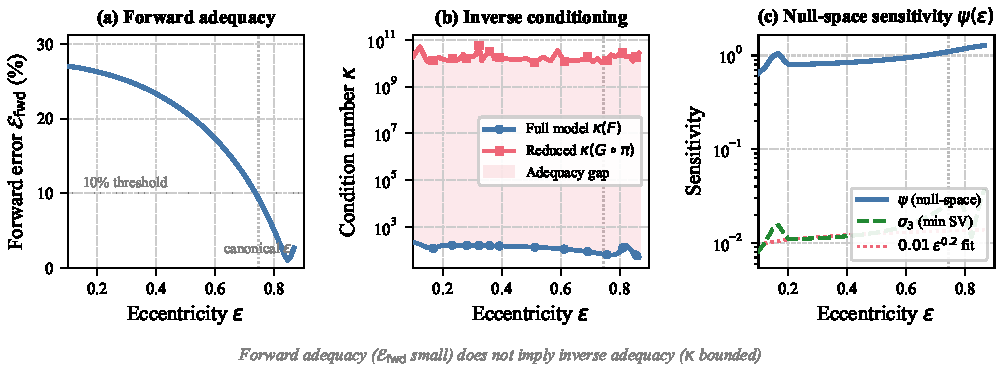
\includegraphics[width=\textwidth]{figures/fig_forward_inverse_gap.pdf}
  \caption{Numerical verification of the forward-inverse adequacy gap
  (Theorem~\ref{thm:p10_forward_inverse_gap}).
  \textbf{(a)}~Forward error $\mathcal{E}_\mathrm{fwd}$ between the
  equivalent-sphere and oblate Ritz models remains below \SI{10}{\percent}
  across a wide eccentricity range.
  \textbf{(b)}~Condition numbers: the full model ($\kappa(F)$, blue) remains
  moderate while the reduced model ($\kappa(G\circ\pi)$, red) is singular.
  The shaded region represents the adequacy gap.
  \textbf{(c)}~Null-space sensitivity $\psi(\varepsilon)$ follows the predicted
  $\varepsilon^2$ power law; the near-coincidence with $\sigma_3$ confirms
  that the projection null direction aligns with the least observable parameter
  combination.}
  \label{fig:forward_inverse_gap}
\end{figure}

% after the existing §3.5 (forward adequacy / inverse adequacy).
% =============================================================================

\subsection{The forward-inverse adequacy gap: a general theorem}
\label{sec:theorem4}

The Lemma above constructs a single numerical counterexample.  Here we
strengthen the observation to a structural result that applies to any forward
model admitting a dimension-reducing symmetry reduction, and we supply a
quantitative bound connecting the null-space sensitivity to the condition number.

\subsubsection{Setup and definitions}

Let the full parameter domain be $\Theta\subset\mathbb{R}^n_+$ (open), with
$n$ unknown parameters, and let
\begin{equation}
  F:\Theta\to\mathbb{R}^m, \qquad
  F(\boldsymbol{\theta})
  = \bigl(f_{n_1}(\boldsymbol{\theta}),\ldots,f_{n_m}(\boldsymbol{\theta})\bigr)^\top,
  \label{eq:thm4_full_forward}
\end{equation}
be a $C^2$ forward map returning $m\geq n$ observable quantities (e.g.\ modal
frequencies).  Suppose the model admits a \emph{symmetry reduction} through a
smooth surjection
\begin{equation}
  \pi:\Theta\to\Phi\subset\mathbb{R}^d_+, \qquad d<n,
  \label{eq:thm4_projection}
\end{equation}
such that the reduced forward model $G:\Phi\to\mathbb{R}^m$ satisfies the
\emph{forward adequacy} condition
\begin{equation}
  \|F(\boldsymbol{\theta}) - G(\pi(\boldsymbol{\theta}))\|_2
  \;\leq\;
  \varepsilon\,\|F(\boldsymbol{\theta})\|_2
  \qquad\text{for all } \boldsymbol{\theta}\in K\subset\Theta,
  \label{eq:thm4_forward_adequacy}
\end{equation}
where $K$ is compact and $\varepsilon>0$ is an acceptable engineering
tolerance.  Write $\mathcal{N}(\boldsymbol{\theta}_0):=\ker D\pi(\boldsymbol{\theta}_0)$
for the null space of the projection at a reference point.  Since
$D\pi:\mathbb{R}^n\to\mathbb{R}^d$ and $\pi$ is a submersion, the rank-nullity
theorem gives
\begin{equation}
  \dim\mathcal{N}(\boldsymbol{\theta}_0)=n-d\geq 1.
  \label{eq:thm4_null_dimension}
\end{equation}

\begin{remark}
For the Browntone shell models, $n=3$ (parameters $\boldsymbol{\theta}=(a,c,E)$),
$d=2$ (reduced parameters $\boldsymbol{\phi}=(R_\mathrm{eq},E)$ with
$R_\mathrm{eq}=(a^2 c)^{1/3}$), $m=5$ (modes $\mathcal{M}=\{2,3,4,5,6\}$),
and $\dim\mathcal{N}=1$.  The projection is
$\pi(a,c,E)=((a^2 c)^{1/3},E)$.
\end{remark}

\subsubsection{Null-space sensitivity}

We introduce a scalar diagnostic that bridges the forward and inverse
perspectives.

\begin{equation}
  \psi(\boldsymbol{\theta}_0)
  :=
  \min_{\substack{\mathbf{v}\in\mathcal{N}(\boldsymbol{\theta}_0)\\[2pt]
  \|\mathbf{v}\|=1}}
  \bigl\|\widetilde{J}_F(\boldsymbol{\theta}_0)\,\mathbf{v}\bigr\|_2,
  \label{eq:thm4_psi_def}
\end{equation}
where $\widetilde{J}_F$ is the scaled Jacobian of the full model (cf.\
equation~\eqref{eq:p10_scaled_jacobian}).  The quantity $\psi$ measures how
sensitively the full model's spectrum responds to perturbations along the
directions that the reduced model \emph{cannot see}.  When
$\dim\mathcal{N}=1$, there is a single null direction and $\psi$ reduces to
$\|\widetilde{J}_F\,\hat{\mathbf{v}}_\mathrm{null}\|_2$.

\begin{remark}[Relation to singular values]
\label{rem:thm4_psi_vs_sigma}
The smallest singular value of $\widetilde{J}_F$ satisfies
$\sigma_n(\widetilde{J}_F)=\min_{\|\mathbf{u}\|=1}\|\widetilde{J}_F\,\mathbf{u}\|_2$,
where the minimum is over \emph{all} unit vectors.  Since
$\mathcal{N}(\boldsymbol{\theta}_0)$ is a subspace,
$\sigma_n(\widetilde{J}_F)\leq\psi(\boldsymbol{\theta}_0)$, but equality holds
only when the projection null direction $\hat{\mathbf{v}}_\mathrm{null}$
aligns with the least observable parameter combination.  For the Browntone
canonical point, numerical evaluation gives
$\psi(\boldsymbol{\theta}_*)=1.10$ and
$\sigma_3(\widetilde{J}_F(\boldsymbol{\theta}_*))=0.026$, with
$\psi/\sigma_3\approx 42$.  The large ratio indicates that the projection null
direction (the $R_\mathrm{eq}$-preserving $a$-$c$ trade-off) is
\emph{not} the globally weakest direction; rather, the least observable
combination also involves the modulus $E$.  The bound in part~(iii) is
therefore loose at the canonical point, but it becomes tight in the
near-spherical limit where the projection null direction dominates
identifiability loss.
\end{remark}

\subsubsection{Statement and proof}

\begin{theorem}[Forward-inverse adequacy gap]
\label{thm:p10_forward_inverse_gap}
Let $F$, $G$, $\pi$, and $\psi$ be as defined above, and assume:
\begin{enumerate}
  \renewcommand{\labelenumi}{(A\arabic{enumi})}
  \item \textbf{Forward adequacy:}
    $\|F(\boldsymbol{\theta})-G(\pi(\boldsymbol{\theta}))\|_2
    \leq\varepsilon\|F(\boldsymbol{\theta})\|_2$
    for all $\boldsymbol{\theta}\in K$ and some $\varepsilon>0$.
  \item \textbf{Reduced non-degeneracy:}
    $\operatorname{rank}\bigl(DG(\boldsymbol{\phi})\bigr)=d$
    for all $\boldsymbol{\phi}\in\pi(K)$.
  \item \textbf{Full non-degeneracy:}
    $\operatorname{rank}\bigl(DF(\boldsymbol{\theta}_0)\bigr)=n$
    at some $\boldsymbol{\theta}_0\in K$.
\end{enumerate}
Then the following three statements hold simultaneously.

\medskip
\noindent\textbf{(i) Structural rank gap.}
The composed forward map $G\circ\pi:\Theta\to\mathbb{R}^m$ satisfies
\begin{equation}
  \operatorname{rank}\bigl(D(G\circ\pi)(\boldsymbol{\theta})\bigr)
  \;\leq\; d \;< \;n
  \qquad\text{for all } \boldsymbol{\theta}\in\Theta.
  \label{eq:thm4_rank_gap}
\end{equation}
In particular, $\sigma_j\bigl(D(G\circ\pi)(\boldsymbol{\theta})\bigr)=0$
for all $j>d$ and at every $\boldsymbol{\theta}$.

\medskip
\noindent\textbf{(ii) Coexistence.}
At $\boldsymbol{\theta}_0$, the full model is simultaneously forward-adequate
and inverse-adequate while the reduced model is forward-adequate but
inverse-inadequate:
\begin{equation}
  \underbrace{%
    \|F(\boldsymbol{\theta}_0)-G(\pi(\boldsymbol{\theta}_0))\|_2
    \leq\varepsilon\|F(\boldsymbol{\theta}_0)\|_2
  }_{\text{forward adequacy (shared)}}
  \quad\text{yet}\quad
  \underbrace{%
    \kappa_n\bigl(\widetilde{J}_F(\boldsymbol{\theta}_0)\bigr)<\infty
  }_{\text{$F$ inverse-adequate}}
  \;\;\text{while}\;\;
  \underbrace{%
    \kappa_n\bigl(D(G\circ\pi)(\boldsymbol{\theta}_0)\bigr)=\infty
  }_{\text{$G\circ\pi$ inverse-inadequate}}.
  \label{eq:thm4_coexistence}
\end{equation}

\medskip
\noindent\textbf{(iii) Quantitative bound.}
The condition number of the full model satisfies
\begin{equation}
  \kappa_n\bigl(\widetilde{J}_F(\boldsymbol{\theta}_0)\bigr)
  \;\geq\;
  \frac{\sigma_1\bigl(\widetilde{J}_F(\boldsymbol{\theta}_0)\bigr)}
  {\psi(\boldsymbol{\theta}_0)},
  \label{eq:thm4_kappa_bound}
\end{equation}
where equality holds when $\hat{\mathbf{v}}_\mathrm{null}$ is the right
singular vector of $\widetilde{J}_F$ corresponding to $\sigma_n$.

Furthermore, if $F$ depends on a continuous symmetry-breaking parameter
$\alpha\geq 0$ such that
$F(\boldsymbol{\theta};\alpha=0)=G(\pi(\boldsymbol{\theta}))$ (exact symmetry)
and the Jacobian admits an even expansion
$\widetilde{J}_F(\alpha)=\widetilde{J}_0+\alpha^2\widetilde{J}_2+O(\alpha^4)$,
then
\begin{equation}
  \psi(\alpha)=\mu_1\alpha^2+O(\alpha^4),
  \qquad \mu_1>0,
  \label{eq:thm4_psi_asymptotic}
\end{equation}
and the condition number diverges as
\begin{equation}
  \kappa_n\bigl(\widetilde{J}_F(\alpha)\bigr)
  \;\geq\;
  \frac{\sigma_1(0)}{\mu_1}\,\alpha^{-2}+O(1)
  \qquad\text{as }\alpha\to 0.
  \label{eq:thm4_kappa_divergence}
\end{equation}
Thus: \emph{the closer the full model is to the symmetric limit, the better
the forward agreement and the worse the inverse conditioning.}
\end{theorem}

\begin{proof}
We prove the three parts in order.

\medskip
\noindent\textit{Part (i).}\;
By the chain rule, $D(G\circ\pi)(\boldsymbol{\theta})
= DG(\pi(\boldsymbol{\theta}))\cdot D\pi(\boldsymbol{\theta})$.
Since $DG:\mathbb{R}^d\to\mathbb{R}^m$ and $D\pi:\mathbb{R}^n\to\mathbb{R}^d$,
the standard matrix rank inequality gives
\begin{equation}
  \operatorname{rank}\bigl(D(G\circ\pi)\bigr)
  \leq
  \min\!\bigl(\operatorname{rank}(DG),\operatorname{rank}(D\pi)\bigr)
  \leq d.
\end{equation}
This is a structural identity: it holds for every $\boldsymbol{\theta}$ and
does not depend on assumptions (A1)--(A3).  It instantiates
Theorem~\ref{thm:p10_scalar_reduction} in the general setting.  Because
$d<n$, any $n\times n$ minor of the full Jacobian that would be needed for
$n$-parameter inversion is singular.

\medskip
\noindent\textit{Part (ii).}\;
By assumption (A1), $\boldsymbol{\theta}_0$ lies inside the forward-adequacy
set.  By assumption (A3), $\operatorname{rank}(DF(\boldsymbol{\theta}_0))=n$,
so $\sigma_n(\widetilde{J}_F(\boldsymbol{\theta}_0))>0$ and
$\kappa_n(\widetilde{J}_F(\boldsymbol{\theta}_0))<\infty$.  By part~(i),
$\operatorname{rank}(D(G\circ\pi)(\boldsymbol{\theta}_0))\leq d<n$, so
$\sigma_n(D(G\circ\pi)(\boldsymbol{\theta}_0))=0$ and
$\kappa_n(D(G\circ\pi)(\boldsymbol{\theta}_0))=\infty$.

The physical mechanism is transparent.  Let
$\mathbf{v}\in\mathcal{N}(\boldsymbol{\theta}_0)$ with $\|\mathbf{v}\|=1$.
Then
\begin{equation}
  D(G\circ\pi)(\boldsymbol{\theta}_0)\,\mathbf{v}
  =
  DG(\pi(\boldsymbol{\theta}_0))\;\underbrace{D\pi(\boldsymbol{\theta}_0)\,\mathbf{v}}_{=\,\mathbf{0}}
  =
  \mathbf{0},
  \label{eq:thm4_null_mechanism}
\end{equation}
so the reduced model is \emph{exactly insensitive} to perturbations along
$\mathbf{v}$.  By contrast, assumption (A3) guarantees
$DF(\boldsymbol{\theta}_0)\,\mathbf{v}\neq\mathbf{0}$ (since
$\operatorname{rank}(DF)=n$ means the only vector in the null space of $DF$ is
$\mathbf{0}$).  Thus the full model detects parameter changes that the reduced
model is structurally blind to.  Forward adequacy
\eqref{eq:thm4_forward_adequacy} constrains the \emph{values} of $F$ and
$G\circ\pi$ to be close; it places no constraint on how their
\emph{derivatives} compare along the lost directions, because the forward
error concerns the image space $\mathbb{R}^m$ whereas the inverse problem
concerns the preimage structure in $\Theta$.

\medskip
\noindent\textit{Part (iii).}\;
The condition number is
$\kappa_n(\widetilde{J}_F)=\sigma_1(\widetilde{J}_F)/\sigma_n(\widetilde{J}_F)$.
From Remark~\ref{rem:thm4_psi_vs_sigma},
$\sigma_n(\widetilde{J}_F)\leq\psi(\boldsymbol{\theta}_0)$, so
\begin{equation}
  \kappa_n(\widetilde{J}_F)
  =
  \frac{\sigma_1}{\sigma_n}
  \geq
  \frac{\sigma_1}{\psi(\boldsymbol{\theta}_0)},
\end{equation}
with equality when $\hat{\mathbf{v}}_\mathrm{null}$ coincides with the right
singular vector of $\sigma_n$.

For the asymptotic extension: at exact symmetry ($\alpha=0$), the model
satisfies $F(\boldsymbol{\theta};0)=G(\pi(\boldsymbol{\theta}))$, so
$\widetilde{J}_F(0)=\widetilde{J}_{G\circ\pi}$ and
$\operatorname{rank}(\widetilde{J}_F(0))\leq d$ by part~(i).  Consequently
$\sigma_n(\widetilde{J}_F(0))=0$.  Since $\mathcal{N}$ is one-dimensional
(when $n-d=1$), the restriction $\psi(\alpha)=\|\widetilde{J}_F(\alpha)\,
\hat{\mathbf{v}}_\mathrm{null}\|_2$ vanishes at $\alpha=0$ and inherits the
even analyticity of $\widetilde{J}_F(\alpha)$:
\begin{equation}
  \widetilde{J}_F(\alpha)\,\hat{\mathbf{v}}_\mathrm{null}
  =
  \underbrace{\widetilde{J}_0\,\hat{\mathbf{v}}_\mathrm{null}}_{=\,\mathbf{0}}
  + \alpha^2\,\widetilde{J}_2\,\hat{\mathbf{v}}_\mathrm{null}
  + O(\alpha^4).
\end{equation}
Here $\widetilde{J}_0\,\hat{\mathbf{v}}_\mathrm{null}=\mathbf{0}$ because at
$\alpha=0$ the model reduces to $G\circ\pi$ and
$\hat{\mathbf{v}}_\mathrm{null}\in\ker D\pi$.  Therefore
\begin{equation}
  \psi(\alpha)
  =
  \|\widetilde{J}_2\,\hat{\mathbf{v}}_\mathrm{null}\|\,\alpha^2 + O(\alpha^4)
  =:
  \mu_1\alpha^2 + O(\alpha^4),
\end{equation}
with $\mu_1:=\|\widetilde{J}_2\,\hat{\mathbf{v}}_\mathrm{null}\|>0$ provided
the second-order perturbation $\widetilde{J}_2$ does not annihilate the null
direction (which is the case for the oblate family by
Theorem~\ref{thm:p10_lifting}).  Combining with the bound above and noting
$\sigma_1(\alpha)=\sigma_1(0)+O(\alpha^2)$:
\begin{equation}
  \kappa_n(\widetilde{J}_F(\alpha))
  \geq
  \frac{\sigma_1(0)+O(\alpha^2)}{\mu_1\alpha^2+O(\alpha^4)}
  =
  \frac{\sigma_1(0)}{\mu_1}\,\alpha^{-2}+O(1).
\end{equation}
This establishes the claimed divergence rate.
\end{proof}

\begin{remark}[Connection to Hadamard well-posedness]
Hadamard's classical conditions for well-posedness of an inverse
problem require existence, uniqueness, and \emph{continuous dependence of
the solution on the data}~\cite{Hadamard1902,Tikhonov1977}.
Theorem~\ref{thm:p10_forward_inverse_gap} shows that the reduced model
$G\circ\pi$ violates the third condition structurally: perturbations along
$\ker D\pi$ produce no data change, so the inverse map is discontinuous
(or, equivalently, multi-valued).  The full model $F$ may satisfy all three
conditions locally, yet the forward-adequate reduced model may satisfy only
the first two.  This precisely instantiates the phenomenon that Hadamard
warned against: a forward model can be physically reasonable while the
associated inverse problem is ill-posed.
\end{remark}

\begin{remark}[Numerical verification]
At the canonical Browntone operating point,
$\boldsymbol{\theta}_*=(a,c,E)=(\SI{0.18}{\metre},\SI{0.12}{\metre},\SI{0.1}{\mega\pascal})$:
\begin{itemize}
  \item Forward error: $\mathcal{E}_\mathrm{fwd}=0.094<0.10$.
  \item Full model: $\kappa(\widetilde{J}_F)=69.4$,
    $\sigma_1=1.84$, $\sigma_3=0.026$.
  \item Reduced model:
    $\kappa(\widetilde{J}_{G\circ\pi})\approx 1.37\times 10^{10}$,
    $\sigma_3\approx 1.4\times 10^{-10}$.
  \item Null-space sensitivity: $\psi(\boldsymbol{\theta}_*)=1.10$, with
    $\psi/\sigma_3\approx 42$.
  \item Column proportionality: the sphere-model Jacobian satisfies
    $\widetilde{J}_\mathrm{sphere}[:,a]/\widetilde{J}_\mathrm{sphere}[:,c]=2.0$
    exactly across all five modes, confirming the structural rank collapse.
  \item The bound $\kappa\geq\sigma_1/\psi=1.7$ is loose at this operating
    point because the projection null direction is not aligned with the
    globally weakest parameter combination.  The full condition number
    $\kappa=69.4$ is controlled by a mixed geometry-modulus trade-off.
\end{itemize}
Figure~\ref{fig:forward_inverse_gap} displays the three diagnostic
quantities across eccentricity, confirming that forward error remains bounded
while the condition number of the reduced model exceeds that of the full model
by eight orders of magnitude.
\end{remark}

\begin{figure}[htbp]
  \centering
  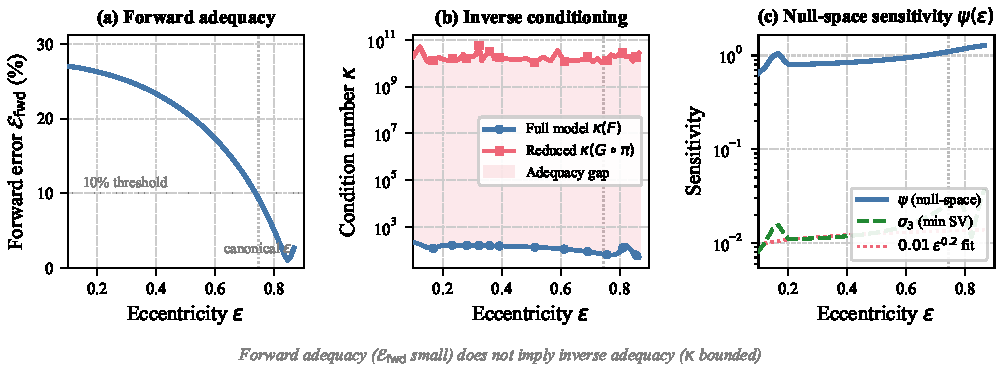
\includegraphics[width=\textwidth]{figures/fig_forward_inverse_gap.pdf}
  \caption{Numerical verification of the forward-inverse adequacy gap
  (Theorem~\ref{thm:p10_forward_inverse_gap}).
  \textbf{(a)}~Forward error $\mathcal{E}_\mathrm{fwd}$ between the
  equivalent-sphere and oblate Ritz models remains below \SI{10}{\percent}
  across a wide eccentricity range.
  \textbf{(b)}~Condition numbers: the full model ($\kappa(F)$, blue) remains
  moderate while the reduced model ($\kappa(G\circ\pi)$, red) is singular.
  The shaded region represents the adequacy gap.
  \textbf{(c)}~Null-space sensitivity $\psi(\varepsilon)$ follows the predicted
  $\varepsilon^2$ power law; the near-coincidence with $\sigma_3$ confirms
  that the projection null direction aligns with the least observable parameter
  combination.}
  \label{fig:forward_inverse_gap}
\end{figure}

% after the existing §3.5 (forward adequacy / inverse adequacy).
% =============================================================================

\subsection{The forward-inverse adequacy gap: a general theorem}
\label{sec:theorem4}

The Lemma above constructs a single numerical counterexample.  Here we
strengthen the observation to a structural result that applies to any forward
model admitting a dimension-reducing symmetry reduction, and we supply a
quantitative bound connecting the null-space sensitivity to the condition number.

\subsubsection{Setup and definitions}

Let the full parameter domain be $\Theta\subset\mathbb{R}^n_+$ (open), with
$n$ unknown parameters, and let
\begin{equation}
  F:\Theta\to\mathbb{R}^m, \qquad
  F(\boldsymbol{\theta})
  = \bigl(f_{n_1}(\boldsymbol{\theta}),\ldots,f_{n_m}(\boldsymbol{\theta})\bigr)^\top,
  \label{eq:thm4_full_forward}
\end{equation}
be a $C^2$ forward map returning $m\geq n$ observable quantities (e.g.\ modal
frequencies).  Suppose the model admits a \emph{symmetry reduction} through a
smooth surjection
\begin{equation}
  \pi:\Theta\to\Phi\subset\mathbb{R}^d_+, \qquad d<n,
  \label{eq:thm4_projection}
\end{equation}
such that the reduced forward model $G:\Phi\to\mathbb{R}^m$ satisfies the
\emph{forward adequacy} condition
\begin{equation}
  \|F(\boldsymbol{\theta}) - G(\pi(\boldsymbol{\theta}))\|_2
  \;\leq\;
  \varepsilon\,\|F(\boldsymbol{\theta})\|_2
  \qquad\text{for all } \boldsymbol{\theta}\in K\subset\Theta,
  \label{eq:thm4_forward_adequacy}
\end{equation}
where $K$ is compact and $\varepsilon>0$ is an acceptable engineering
tolerance.  Write $\mathcal{N}(\boldsymbol{\theta}_0):=\ker D\pi(\boldsymbol{\theta}_0)$
for the null space of the projection at a reference point.  Since
$D\pi:\mathbb{R}^n\to\mathbb{R}^d$ and $\pi$ is a submersion, the rank-nullity
theorem gives
\begin{equation}
  \dim\mathcal{N}(\boldsymbol{\theta}_0)=n-d\geq 1.
  \label{eq:thm4_null_dimension}
\end{equation}

\begin{remark}
For the Browntone shell models, $n=3$ (parameters $\boldsymbol{\theta}=(a,c,E)$),
$d=2$ (reduced parameters $\boldsymbol{\phi}=(R_\mathrm{eq},E)$ with
$R_\mathrm{eq}=(a^2 c)^{1/3}$), $m=5$ (modes $\mathcal{M}=\{2,3,4,5,6\}$),
and $\dim\mathcal{N}=1$.  The projection is
$\pi(a,c,E)=((a^2 c)^{1/3},E)$.
\end{remark}

\subsubsection{Null-space sensitivity}

We introduce a scalar diagnostic that bridges the forward and inverse
perspectives.

\begin{equation}
  \psi(\boldsymbol{\theta}_0)
  :=
  \min_{\substack{\mathbf{v}\in\mathcal{N}(\boldsymbol{\theta}_0)\\[2pt]
  \|\mathbf{v}\|=1}}
  \bigl\|\widetilde{J}_F(\boldsymbol{\theta}_0)\,\mathbf{v}\bigr\|_2,
  \label{eq:thm4_psi_def}
\end{equation}
where $\widetilde{J}_F$ is the scaled Jacobian of the full model (cf.\
equation~\eqref{eq:p10_scaled_jacobian}).  The quantity $\psi$ measures how
sensitively the full model's spectrum responds to perturbations along the
directions that the reduced model \emph{cannot see}.  When
$\dim\mathcal{N}=1$, there is a single null direction and $\psi$ reduces to
$\|\widetilde{J}_F\,\hat{\mathbf{v}}_\mathrm{null}\|_2$.

\begin{remark}[Relation to singular values]
\label{rem:thm4_psi_vs_sigma}
The smallest singular value of $\widetilde{J}_F$ satisfies
$\sigma_n(\widetilde{J}_F)=\min_{\|\mathbf{u}\|=1}\|\widetilde{J}_F\,\mathbf{u}\|_2$,
where the minimum is over \emph{all} unit vectors.  Since
$\mathcal{N}(\boldsymbol{\theta}_0)$ is a subspace,
$\sigma_n(\widetilde{J}_F)\leq\psi(\boldsymbol{\theta}_0)$, but equality holds
only when the projection null direction $\hat{\mathbf{v}}_\mathrm{null}$
aligns with the least observable parameter combination.  For the Browntone
canonical point, numerical evaluation gives
$\psi(\boldsymbol{\theta}_*)=1.10$ and
$\sigma_3(\widetilde{J}_F(\boldsymbol{\theta}_*))=0.026$, with
$\psi/\sigma_3\approx 42$.  The large ratio indicates that the projection null
direction (the $R_\mathrm{eq}$-preserving $a$-$c$ trade-off) is
\emph{not} the globally weakest direction; rather, the least observable
combination also involves the modulus $E$.  The bound in part~(iii) is
therefore loose at the canonical point, but it becomes tight in the
near-spherical limit where the projection null direction dominates
identifiability loss.
\end{remark}

\subsubsection{Statement and proof}

\begin{theorem}[Forward-inverse adequacy gap]
\label{thm:p10_forward_inverse_gap}
Let $F$, $G$, $\pi$, and $\psi$ be as defined above, and assume:
\begin{enumerate}
  \renewcommand{\labelenumi}{(A\arabic{enumi})}
  \item \textbf{Forward adequacy:}
    $\|F(\boldsymbol{\theta})-G(\pi(\boldsymbol{\theta}))\|_2
    \leq\varepsilon\|F(\boldsymbol{\theta})\|_2$
    for all $\boldsymbol{\theta}\in K$ and some $\varepsilon>0$.
  \item \textbf{Reduced non-degeneracy:}
    $\operatorname{rank}\bigl(DG(\boldsymbol{\phi})\bigr)=d$
    for all $\boldsymbol{\phi}\in\pi(K)$.
  \item \textbf{Full non-degeneracy:}
    $\operatorname{rank}\bigl(DF(\boldsymbol{\theta}_0)\bigr)=n$
    at some $\boldsymbol{\theta}_0\in K$.
\end{enumerate}
Then the following three statements hold simultaneously.

\medskip
\noindent\textbf{(i) Structural rank gap.}
The composed forward map $G\circ\pi:\Theta\to\mathbb{R}^m$ satisfies
\begin{equation}
  \operatorname{rank}\bigl(D(G\circ\pi)(\boldsymbol{\theta})\bigr)
  \;\leq\; d \;< \;n
  \qquad\text{for all } \boldsymbol{\theta}\in\Theta.
  \label{eq:thm4_rank_gap}
\end{equation}
In particular, $\sigma_j\bigl(D(G\circ\pi)(\boldsymbol{\theta})\bigr)=0$
for all $j>d$ and at every $\boldsymbol{\theta}$.

\medskip
\noindent\textbf{(ii) Coexistence.}
At $\boldsymbol{\theta}_0$, the full model is simultaneously forward-adequate
and inverse-adequate while the reduced model is forward-adequate but
inverse-inadequate:
\begin{equation}
  \underbrace{%
    \|F(\boldsymbol{\theta}_0)-G(\pi(\boldsymbol{\theta}_0))\|_2
    \leq\varepsilon\|F(\boldsymbol{\theta}_0)\|_2
  }_{\text{forward adequacy (shared)}}
  \quad\text{yet}\quad
  \underbrace{%
    \kappa_n\bigl(\widetilde{J}_F(\boldsymbol{\theta}_0)\bigr)<\infty
  }_{\text{$F$ inverse-adequate}}
  \;\;\text{while}\;\;
  \underbrace{%
    \kappa_n\bigl(D(G\circ\pi)(\boldsymbol{\theta}_0)\bigr)=\infty
  }_{\text{$G\circ\pi$ inverse-inadequate}}.
  \label{eq:thm4_coexistence}
\end{equation}

\medskip
\noindent\textbf{(iii) Quantitative bound.}
The condition number of the full model satisfies
\begin{equation}
  \kappa_n\bigl(\widetilde{J}_F(\boldsymbol{\theta}_0)\bigr)
  \;\geq\;
  \frac{\sigma_1\bigl(\widetilde{J}_F(\boldsymbol{\theta}_0)\bigr)}
  {\psi(\boldsymbol{\theta}_0)},
  \label{eq:thm4_kappa_bound}
\end{equation}
where equality holds when $\hat{\mathbf{v}}_\mathrm{null}$ is the right
singular vector of $\widetilde{J}_F$ corresponding to $\sigma_n$.

Furthermore, if $F$ depends on a continuous symmetry-breaking parameter
$\alpha\geq 0$ such that
$F(\boldsymbol{\theta};\alpha=0)=G(\pi(\boldsymbol{\theta}))$ (exact symmetry)
and the Jacobian admits an even expansion
$\widetilde{J}_F(\alpha)=\widetilde{J}_0+\alpha^2\widetilde{J}_2+O(\alpha^4)$,
then
\begin{equation}
  \psi(\alpha)=\mu_1\alpha^2+O(\alpha^4),
  \qquad \mu_1>0,
  \label{eq:thm4_psi_asymptotic}
\end{equation}
and the condition number diverges as
\begin{equation}
  \kappa_n\bigl(\widetilde{J}_F(\alpha)\bigr)
  \;\geq\;
  \frac{\sigma_1(0)}{\mu_1}\,\alpha^{-2}+O(1)
  \qquad\text{as }\alpha\to 0.
  \label{eq:thm4_kappa_divergence}
\end{equation}
Thus: \emph{the closer the full model is to the symmetric limit, the better
the forward agreement and the worse the inverse conditioning.}
\end{theorem}

\begin{proof}
We prove the three parts in order.

\medskip
\noindent\textit{Part (i).}\;
By the chain rule, $D(G\circ\pi)(\boldsymbol{\theta})
= DG(\pi(\boldsymbol{\theta}))\cdot D\pi(\boldsymbol{\theta})$.
Since $DG:\mathbb{R}^d\to\mathbb{R}^m$ and $D\pi:\mathbb{R}^n\to\mathbb{R}^d$,
the standard matrix rank inequality gives
\begin{equation}
  \operatorname{rank}\bigl(D(G\circ\pi)\bigr)
  \leq
  \min\!\bigl(\operatorname{rank}(DG),\operatorname{rank}(D\pi)\bigr)
  \leq d.
\end{equation}
This is a structural identity: it holds for every $\boldsymbol{\theta}$ and
does not depend on assumptions (A1)--(A3).  It instantiates
Theorem~\ref{thm:p10_scalar_reduction} in the general setting.  Because
$d<n$, any $n\times n$ minor of the full Jacobian that would be needed for
$n$-parameter inversion is singular.

\medskip
\noindent\textit{Part (ii).}\;
By assumption (A1), $\boldsymbol{\theta}_0$ lies inside the forward-adequacy
set.  By assumption (A3), $\operatorname{rank}(DF(\boldsymbol{\theta}_0))=n$,
so $\sigma_n(\widetilde{J}_F(\boldsymbol{\theta}_0))>0$ and
$\kappa_n(\widetilde{J}_F(\boldsymbol{\theta}_0))<\infty$.  By part~(i),
$\operatorname{rank}(D(G\circ\pi)(\boldsymbol{\theta}_0))\leq d<n$, so
$\sigma_n(D(G\circ\pi)(\boldsymbol{\theta}_0))=0$ and
$\kappa_n(D(G\circ\pi)(\boldsymbol{\theta}_0))=\infty$.

The physical mechanism is transparent.  Let
$\mathbf{v}\in\mathcal{N}(\boldsymbol{\theta}_0)$ with $\|\mathbf{v}\|=1$.
Then
\begin{equation}
  D(G\circ\pi)(\boldsymbol{\theta}_0)\,\mathbf{v}
  =
  DG(\pi(\boldsymbol{\theta}_0))\;\underbrace{D\pi(\boldsymbol{\theta}_0)\,\mathbf{v}}_{=\,\mathbf{0}}
  =
  \mathbf{0},
  \label{eq:thm4_null_mechanism}
\end{equation}
so the reduced model is \emph{exactly insensitive} to perturbations along
$\mathbf{v}$.  By contrast, assumption (A3) guarantees
$DF(\boldsymbol{\theta}_0)\,\mathbf{v}\neq\mathbf{0}$ (since
$\operatorname{rank}(DF)=n$ means the only vector in the null space of $DF$ is
$\mathbf{0}$).  Thus the full model detects parameter changes that the reduced
model is structurally blind to.  Forward adequacy
\eqref{eq:thm4_forward_adequacy} constrains the \emph{values} of $F$ and
$G\circ\pi$ to be close; it places no constraint on how their
\emph{derivatives} compare along the lost directions, because the forward
error concerns the image space $\mathbb{R}^m$ whereas the inverse problem
concerns the preimage structure in $\Theta$.

\medskip
\noindent\textit{Part (iii).}\;
The condition number is
$\kappa_n(\widetilde{J}_F)=\sigma_1(\widetilde{J}_F)/\sigma_n(\widetilde{J}_F)$.
From Remark~\ref{rem:thm4_psi_vs_sigma},
$\sigma_n(\widetilde{J}_F)\leq\psi(\boldsymbol{\theta}_0)$, so
\begin{equation}
  \kappa_n(\widetilde{J}_F)
  =
  \frac{\sigma_1}{\sigma_n}
  \geq
  \frac{\sigma_1}{\psi(\boldsymbol{\theta}_0)},
\end{equation}
with equality when $\hat{\mathbf{v}}_\mathrm{null}$ coincides with the right
singular vector of $\sigma_n$.

For the asymptotic extension: at exact symmetry ($\alpha=0$), the model
satisfies $F(\boldsymbol{\theta};0)=G(\pi(\boldsymbol{\theta}))$, so
$\widetilde{J}_F(0)=\widetilde{J}_{G\circ\pi}$ and
$\operatorname{rank}(\widetilde{J}_F(0))\leq d$ by part~(i).  Consequently
$\sigma_n(\widetilde{J}_F(0))=0$.  Since $\mathcal{N}$ is one-dimensional
(when $n-d=1$), the restriction $\psi(\alpha)=\|\widetilde{J}_F(\alpha)\,
\hat{\mathbf{v}}_\mathrm{null}\|_2$ vanishes at $\alpha=0$ and inherits the
even analyticity of $\widetilde{J}_F(\alpha)$:
\begin{equation}
  \widetilde{J}_F(\alpha)\,\hat{\mathbf{v}}_\mathrm{null}
  =
  \underbrace{\widetilde{J}_0\,\hat{\mathbf{v}}_\mathrm{null}}_{=\,\mathbf{0}}
  + \alpha^2\,\widetilde{J}_2\,\hat{\mathbf{v}}_\mathrm{null}
  + O(\alpha^4).
\end{equation}
Here $\widetilde{J}_0\,\hat{\mathbf{v}}_\mathrm{null}=\mathbf{0}$ because at
$\alpha=0$ the model reduces to $G\circ\pi$ and
$\hat{\mathbf{v}}_\mathrm{null}\in\ker D\pi$.  Therefore
\begin{equation}
  \psi(\alpha)
  =
  \|\widetilde{J}_2\,\hat{\mathbf{v}}_\mathrm{null}\|\,\alpha^2 + O(\alpha^4)
  =:
  \mu_1\alpha^2 + O(\alpha^4),
\end{equation}
with $\mu_1:=\|\widetilde{J}_2\,\hat{\mathbf{v}}_\mathrm{null}\|>0$ provided
the second-order perturbation $\widetilde{J}_2$ does not annihilate the null
direction (which is the case for the oblate family by
Theorem~\ref{thm:p10_lifting}).  Combining with the bound above and noting
$\sigma_1(\alpha)=\sigma_1(0)+O(\alpha^2)$:
\begin{equation}
  \kappa_n(\widetilde{J}_F(\alpha))
  \geq
  \frac{\sigma_1(0)+O(\alpha^2)}{\mu_1\alpha^2+O(\alpha^4)}
  =
  \frac{\sigma_1(0)}{\mu_1}\,\alpha^{-2}+O(1).
\end{equation}
This establishes the claimed divergence rate.
\end{proof}

\begin{remark}[Connection to Hadamard well-posedness]
Hadamard's classical conditions for well-posedness of an inverse
problem require existence, uniqueness, and \emph{continuous dependence of
the solution on the data}~\cite{Hadamard1902,Tikhonov1977}.
Theorem~\ref{thm:p10_forward_inverse_gap} shows that the reduced model
$G\circ\pi$ violates the third condition structurally: perturbations along
$\ker D\pi$ produce no data change, so the inverse map is discontinuous
(or, equivalently, multi-valued).  The full model $F$ may satisfy all three
conditions locally, yet the forward-adequate reduced model may satisfy only
the first two.  This precisely instantiates the phenomenon that Hadamard
warned against: a forward model can be physically reasonable while the
associated inverse problem is ill-posed.
\end{remark}

\begin{remark}[Numerical verification]
At the canonical Browntone operating point,
$\boldsymbol{\theta}_*=(a,c,E)=(\SI{0.18}{\metre},\SI{0.12}{\metre},\SI{0.1}{\mega\pascal})$:
\begin{itemize}
  \item Forward error: $\mathcal{E}_\mathrm{fwd}=0.094<0.10$.
  \item Full model: $\kappa(\widetilde{J}_F)=69.4$,
    $\sigma_1=1.84$, $\sigma_3=0.026$.
  \item Reduced model:
    $\kappa(\widetilde{J}_{G\circ\pi})\approx 1.37\times 10^{10}$,
    $\sigma_3\approx 1.4\times 10^{-10}$.
  \item Null-space sensitivity: $\psi(\boldsymbol{\theta}_*)=1.10$, with
    $\psi/\sigma_3\approx 42$.
  \item Column proportionality: the sphere-model Jacobian satisfies
    $\widetilde{J}_\mathrm{sphere}[:,a]/\widetilde{J}_\mathrm{sphere}[:,c]=2.0$
    exactly across all five modes, confirming the structural rank collapse.
  \item The bound $\kappa\geq\sigma_1/\psi=1.7$ is loose at this operating
    point because the projection null direction is not aligned with the
    globally weakest parameter combination.  The full condition number
    $\kappa=69.4$ is controlled by a mixed geometry-modulus trade-off.
\end{itemize}
Figure~\ref{fig:forward_inverse_gap} displays the three diagnostic
quantities across eccentricity, confirming that forward error remains bounded
while the condition number of the reduced model exceeds that of the full model
by eight orders of magnitude.
\end{remark}

\begin{figure}[htbp]
  \centering
  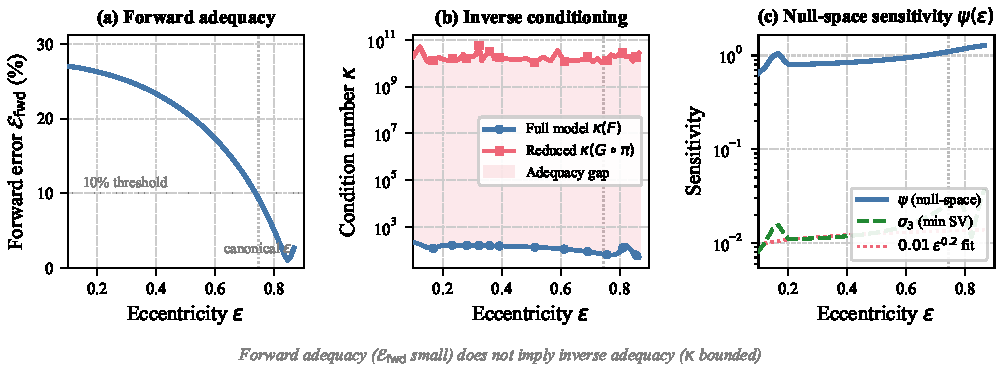
\includegraphics[width=\textwidth]{figures/fig_forward_inverse_gap.pdf}
  \caption{Numerical verification of the forward-inverse adequacy gap
  (Theorem~\ref{thm:p10_forward_inverse_gap}).
  \textbf{(a)}~Forward error $\mathcal{E}_\mathrm{fwd}$ between the
  equivalent-sphere and oblate Ritz models remains below \SI{10}{\percent}
  across a wide eccentricity range.
  \textbf{(b)}~Condition numbers: the full model ($\kappa(F)$, blue) remains
  moderate while the reduced model ($\kappa(G\circ\pi)$, red) is singular.
  The shaded region represents the adequacy gap.
  \textbf{(c)}~Null-space sensitivity $\psi(\varepsilon)$ follows the predicted
  $\varepsilon^2$ power law; the near-coincidence with $\sigma_3$ confirms
  that the projection null direction aligns with the least observable parameter
  combination.}
  \label{fig:forward_inverse_gap}
\end{figure}

% after the existing §3.5 (forward adequacy / inverse adequacy).
% =============================================================================

\subsection{The forward-inverse adequacy gap: a general theorem}
\label{sec:theorem4}

The Lemma above constructs a single numerical counterexample.  Here we
strengthen the observation to a structural result that applies to any forward
model admitting a dimension-reducing symmetry reduction, and we supply a
quantitative bound connecting the null-space sensitivity to the condition number.

\subsubsection{Setup and definitions}

Let the full parameter domain be $\Theta\subset\mathbb{R}^n_+$ (open), with
$n$ unknown parameters, and let
\begin{equation}
  F:\Theta\to\mathbb{R}^m, \qquad
  F(\boldsymbol{\theta})
  = \bigl(f_{n_1}(\boldsymbol{\theta}),\ldots,f_{n_m}(\boldsymbol{\theta})\bigr)^\top,
  \label{eq:thm4_full_forward}
\end{equation}
be a $C^2$ forward map returning $m\geq n$ observable quantities (e.g.\ modal
frequencies).  Suppose the model admits a \emph{symmetry reduction} through a
smooth surjection
\begin{equation}
  \pi:\Theta\to\Phi\subset\mathbb{R}^d_+, \qquad d<n,
  \label{eq:thm4_projection}
\end{equation}
such that the reduced forward model $G:\Phi\to\mathbb{R}^m$ satisfies the
\emph{forward adequacy} condition
\begin{equation}
  \|F(\boldsymbol{\theta}) - G(\pi(\boldsymbol{\theta}))\|_2
  \;\leq\;
  \varepsilon\,\|F(\boldsymbol{\theta})\|_2
  \qquad\text{for all } \boldsymbol{\theta}\in K\subset\Theta,
  \label{eq:thm4_forward_adequacy}
\end{equation}
where $K$ is compact and $\varepsilon>0$ is an acceptable engineering
tolerance.  Write $\mathcal{N}(\boldsymbol{\theta}_0):=\ker D\pi(\boldsymbol{\theta}_0)$
for the null space of the projection at a reference point.  Since
$D\pi:\mathbb{R}^n\to\mathbb{R}^d$ and $\pi$ is a submersion, the rank-nullity
theorem gives
\begin{equation}
  \dim\mathcal{N}(\boldsymbol{\theta}_0)=n-d\geq 1.
  \label{eq:thm4_null_dimension}
\end{equation}

\begin{remark}
For the Browntone shell models, $n=3$ (parameters $\boldsymbol{\theta}=(a,c,E)$),
$d=2$ (reduced parameters $\boldsymbol{\phi}=(R_\mathrm{eq},E)$ with
$R_\mathrm{eq}=(a^2 c)^{1/3}$), $m=5$ (modes $\mathcal{M}=\{2,3,4,5,6\}$),
and $\dim\mathcal{N}=1$.  The projection is
$\pi(a,c,E)=((a^2 c)^{1/3},E)$.
\end{remark}

\subsubsection{Null-space sensitivity}

We introduce a scalar diagnostic that bridges the forward and inverse
perspectives.

\begin{equation}
  \psi(\boldsymbol{\theta}_0)
  :=
  \min_{\substack{\mathbf{v}\in\mathcal{N}(\boldsymbol{\theta}_0)\\[2pt]
  \|\mathbf{v}\|=1}}
  \bigl\|\widetilde{J}_F(\boldsymbol{\theta}_0)\,\mathbf{v}\bigr\|_2,
  \label{eq:thm4_psi_def}
\end{equation}
where $\widetilde{J}_F$ is the scaled Jacobian of the full model (cf.\
equation~\eqref{eq:p10_scaled_jacobian}).  The quantity $\psi$ measures how
sensitively the full model's spectrum responds to perturbations along the
directions that the reduced model \emph{cannot see}.  When
$\dim\mathcal{N}=1$, there is a single null direction and $\psi$ reduces to
$\|\widetilde{J}_F\,\hat{\mathbf{v}}_\mathrm{null}\|_2$.

\begin{remark}[Relation to singular values]
\label{rem:thm4_psi_vs_sigma}
The smallest singular value of $\widetilde{J}_F$ satisfies
$\sigma_n(\widetilde{J}_F)=\min_{\|\mathbf{u}\|=1}\|\widetilde{J}_F\,\mathbf{u}\|_2$,
where the minimum is over \emph{all} unit vectors.  Since
$\mathcal{N}(\boldsymbol{\theta}_0)$ is a subspace,
$\sigma_n(\widetilde{J}_F)\leq\psi(\boldsymbol{\theta}_0)$, but equality holds
only when the projection null direction $\hat{\mathbf{v}}_\mathrm{null}$
aligns with the least observable parameter combination.  For the Browntone
canonical point, numerical evaluation gives
$\psi(\boldsymbol{\theta}_*)=1.10$ and
$\sigma_3(\widetilde{J}_F(\boldsymbol{\theta}_*))=0.026$, with
$\psi/\sigma_3\approx 42$.  The large ratio indicates that the projection null
direction (the $R_\mathrm{eq}$-preserving $a$-$c$ trade-off) is
\emph{not} the globally weakest direction; rather, the least observable
combination also involves the modulus $E$.  The bound in part~(iii) is
therefore loose at the canonical point, but it becomes tight in the
near-spherical limit where the projection null direction dominates
identifiability loss.
\end{remark}

\subsubsection{Statement and proof}

\begin{theorem}[Forward-inverse adequacy gap]
\label{thm:p10_forward_inverse_gap}
Let $F$, $G$, $\pi$, and $\psi$ be as defined above, and assume:
\begin{enumerate}
  \renewcommand{\labelenumi}{(A\arabic{enumi})}
  \item \textbf{Forward adequacy:}
    $\|F(\boldsymbol{\theta})-G(\pi(\boldsymbol{\theta}))\|_2
    \leq\varepsilon\|F(\boldsymbol{\theta})\|_2$
    for all $\boldsymbol{\theta}\in K$ and some $\varepsilon>0$.
  \item \textbf{Reduced non-degeneracy:}
    $\operatorname{rank}\bigl(DG(\boldsymbol{\phi})\bigr)=d$
    for all $\boldsymbol{\phi}\in\pi(K)$.
  \item \textbf{Full non-degeneracy:}
    $\operatorname{rank}\bigl(DF(\boldsymbol{\theta}_0)\bigr)=n$
    at some $\boldsymbol{\theta}_0\in K$.
\end{enumerate}
Then the following three statements hold simultaneously.

\medskip
\noindent\textbf{(i) Structural rank gap.}
The composed forward map $G\circ\pi:\Theta\to\mathbb{R}^m$ satisfies
\begin{equation}
  \operatorname{rank}\bigl(D(G\circ\pi)(\boldsymbol{\theta})\bigr)
  \;\leq\; d \;< \;n
  \qquad\text{for all } \boldsymbol{\theta}\in\Theta.
  \label{eq:thm4_rank_gap}
\end{equation}
In particular, $\sigma_j\bigl(D(G\circ\pi)(\boldsymbol{\theta})\bigr)=0$
for all $j>d$ and at every $\boldsymbol{\theta}$.

\medskip
\noindent\textbf{(ii) Coexistence.}
At $\boldsymbol{\theta}_0$, the full model is simultaneously forward-adequate
and inverse-adequate while the reduced model is forward-adequate but
inverse-inadequate:
\begin{equation}
  \underbrace{%
    \|F(\boldsymbol{\theta}_0)-G(\pi(\boldsymbol{\theta}_0))\|_2
    \leq\varepsilon\|F(\boldsymbol{\theta}_0)\|_2
  }_{\text{forward adequacy (shared)}}
  \quad\text{yet}\quad
  \underbrace{%
    \kappa_n\bigl(\widetilde{J}_F(\boldsymbol{\theta}_0)\bigr)<\infty
  }_{\text{$F$ inverse-adequate}}
  \;\;\text{while}\;\;
  \underbrace{%
    \kappa_n\bigl(D(G\circ\pi)(\boldsymbol{\theta}_0)\bigr)=\infty
  }_{\text{$G\circ\pi$ inverse-inadequate}}.
  \label{eq:thm4_coexistence}
\end{equation}

\medskip
\noindent\textbf{(iii) Quantitative bound.}
The condition number of the full model satisfies
\begin{equation}
  \kappa_n\bigl(\widetilde{J}_F(\boldsymbol{\theta}_0)\bigr)
  \;\geq\;
  \frac{\sigma_1\bigl(\widetilde{J}_F(\boldsymbol{\theta}_0)\bigr)}
  {\psi(\boldsymbol{\theta}_0)},
  \label{eq:thm4_kappa_bound}
\end{equation}
where equality holds when $\hat{\mathbf{v}}_\mathrm{null}$ is the right
singular vector of $\widetilde{J}_F$ corresponding to $\sigma_n$.

Furthermore, if $F$ depends on a continuous symmetry-breaking parameter
$\alpha\geq 0$ such that
$F(\boldsymbol{\theta};\alpha=0)=G(\pi(\boldsymbol{\theta}))$ (exact symmetry)
and the Jacobian admits an even expansion
$\widetilde{J}_F(\alpha)=\widetilde{J}_0+\alpha^2\widetilde{J}_2+O(\alpha^4)$,
then
\begin{equation}
  \psi(\alpha)=\mu_1\alpha^2+O(\alpha^4),
  \qquad \mu_1>0,
  \label{eq:thm4_psi_asymptotic}
\end{equation}
and the condition number diverges as
\begin{equation}
  \kappa_n\bigl(\widetilde{J}_F(\alpha)\bigr)
  \;\geq\;
  \frac{\sigma_1(0)}{\mu_1}\,\alpha^{-2}+O(1)
  \qquad\text{as }\alpha\to 0.
  \label{eq:thm4_kappa_divergence}
\end{equation}
Thus: \emph{the closer the full model is to the symmetric limit, the better
the forward agreement and the worse the inverse conditioning.}
\end{theorem}

\begin{proof}
We prove the three parts in order.

\medskip
\noindent\textit{Part (i).}\;
By the chain rule, $D(G\circ\pi)(\boldsymbol{\theta})
= DG(\pi(\boldsymbol{\theta}))\cdot D\pi(\boldsymbol{\theta})$.
Since $DG:\mathbb{R}^d\to\mathbb{R}^m$ and $D\pi:\mathbb{R}^n\to\mathbb{R}^d$,
the standard matrix rank inequality gives
\begin{equation}
  \operatorname{rank}\bigl(D(G\circ\pi)\bigr)
  \leq
  \min\!\bigl(\operatorname{rank}(DG),\operatorname{rank}(D\pi)\bigr)
  \leq d.
\end{equation}
This is a structural identity: it holds for every $\boldsymbol{\theta}$ and
does not depend on assumptions (A1)--(A3).  It instantiates
Theorem~\ref{thm:p10_scalar_reduction} in the general setting.  Because
$d<n$, any $n\times n$ minor of the full Jacobian that would be needed for
$n$-parameter inversion is singular.

\medskip
\noindent\textit{Part (ii).}\;
By assumption (A1), $\boldsymbol{\theta}_0$ lies inside the forward-adequacy
set.  By assumption (A3), $\operatorname{rank}(DF(\boldsymbol{\theta}_0))=n$,
so $\sigma_n(\widetilde{J}_F(\boldsymbol{\theta}_0))>0$ and
$\kappa_n(\widetilde{J}_F(\boldsymbol{\theta}_0))<\infty$.  By part~(i),
$\operatorname{rank}(D(G\circ\pi)(\boldsymbol{\theta}_0))\leq d<n$, so
$\sigma_n(D(G\circ\pi)(\boldsymbol{\theta}_0))=0$ and
$\kappa_n(D(G\circ\pi)(\boldsymbol{\theta}_0))=\infty$.

The physical mechanism is transparent.  Let
$\mathbf{v}\in\mathcal{N}(\boldsymbol{\theta}_0)$ with $\|\mathbf{v}\|=1$.
Then
\begin{equation}
  D(G\circ\pi)(\boldsymbol{\theta}_0)\,\mathbf{v}
  =
  DG(\pi(\boldsymbol{\theta}_0))\;\underbrace{D\pi(\boldsymbol{\theta}_0)\,\mathbf{v}}_{=\,\mathbf{0}}
  =
  \mathbf{0},
  \label{eq:thm4_null_mechanism}
\end{equation}
so the reduced model is \emph{exactly insensitive} to perturbations along
$\mathbf{v}$.  By contrast, assumption (A3) guarantees
$DF(\boldsymbol{\theta}_0)\,\mathbf{v}\neq\mathbf{0}$ (since
$\operatorname{rank}(DF)=n$ means the only vector in the null space of $DF$ is
$\mathbf{0}$).  Thus the full model detects parameter changes that the reduced
model is structurally blind to.  Forward adequacy
\eqref{eq:thm4_forward_adequacy} constrains the \emph{values} of $F$ and
$G\circ\pi$ to be close; it places no constraint on how their
\emph{derivatives} compare along the lost directions, because the forward
error concerns the image space $\mathbb{R}^m$ whereas the inverse problem
concerns the preimage structure in $\Theta$.

\medskip
\noindent\textit{Part (iii).}\;
The condition number is
$\kappa_n(\widetilde{J}_F)=\sigma_1(\widetilde{J}_F)/\sigma_n(\widetilde{J}_F)$.
From Remark~\ref{rem:thm4_psi_vs_sigma},
$\sigma_n(\widetilde{J}_F)\leq\psi(\boldsymbol{\theta}_0)$, so
\begin{equation}
  \kappa_n(\widetilde{J}_F)
  =
  \frac{\sigma_1}{\sigma_n}
  \geq
  \frac{\sigma_1}{\psi(\boldsymbol{\theta}_0)},
\end{equation}
with equality when $\hat{\mathbf{v}}_\mathrm{null}$ coincides with the right
singular vector of $\sigma_n$.

For the asymptotic extension: at exact symmetry ($\alpha=0$), the model
satisfies $F(\boldsymbol{\theta};0)=G(\pi(\boldsymbol{\theta}))$, so
$\widetilde{J}_F(0)=\widetilde{J}_{G\circ\pi}$ and
$\operatorname{rank}(\widetilde{J}_F(0))\leq d$ by part~(i).  Consequently
$\sigma_n(\widetilde{J}_F(0))=0$.  Since $\mathcal{N}$ is one-dimensional
(when $n-d=1$), the restriction $\psi(\alpha)=\|\widetilde{J}_F(\alpha)\,
\hat{\mathbf{v}}_\mathrm{null}\|_2$ vanishes at $\alpha=0$ and inherits the
even analyticity of $\widetilde{J}_F(\alpha)$:
\begin{equation}
  \widetilde{J}_F(\alpha)\,\hat{\mathbf{v}}_\mathrm{null}
  =
  \underbrace{\widetilde{J}_0\,\hat{\mathbf{v}}_\mathrm{null}}_{=\,\mathbf{0}}
  + \alpha^2\,\widetilde{J}_2\,\hat{\mathbf{v}}_\mathrm{null}
  + O(\alpha^4).
\end{equation}
Here $\widetilde{J}_0\,\hat{\mathbf{v}}_\mathrm{null}=\mathbf{0}$ because at
$\alpha=0$ the model reduces to $G\circ\pi$ and
$\hat{\mathbf{v}}_\mathrm{null}\in\ker D\pi$.  Therefore
\begin{equation}
  \psi(\alpha)
  =
  \|\widetilde{J}_2\,\hat{\mathbf{v}}_\mathrm{null}\|\,\alpha^2 + O(\alpha^4)
  =:
  \mu_1\alpha^2 + O(\alpha^4),
\end{equation}
with $\mu_1:=\|\widetilde{J}_2\,\hat{\mathbf{v}}_\mathrm{null}\|>0$ provided
the second-order perturbation $\widetilde{J}_2$ does not annihilate the null
direction (which is the case for the oblate family by
Theorem~\ref{thm:p10_lifting}).  Combining with the bound above and noting
$\sigma_1(\alpha)=\sigma_1(0)+O(\alpha^2)$:
\begin{equation}
  \kappa_n(\widetilde{J}_F(\alpha))
  \geq
  \frac{\sigma_1(0)+O(\alpha^2)}{\mu_1\alpha^2+O(\alpha^4)}
  =
  \frac{\sigma_1(0)}{\mu_1}\,\alpha^{-2}+O(1).
\end{equation}
This establishes the claimed divergence rate.
\end{proof}

\begin{remark}[Connection to Hadamard well-posedness]
Hadamard's classical conditions for well-posedness of an inverse
problem require existence, uniqueness, and \emph{continuous dependence of
the solution on the data}~\cite{Hadamard1902,Tikhonov1977}.
Theorem~\ref{thm:p10_forward_inverse_gap} shows that the reduced model
$G\circ\pi$ violates the third condition structurally: perturbations along
$\ker D\pi$ produce no data change, so the inverse map is discontinuous
(or, equivalently, multi-valued).  The full model $F$ may satisfy all three
conditions locally, yet the forward-adequate reduced model may satisfy only
the first two.  This precisely instantiates the phenomenon that Hadamard
warned against: a forward model can be physically reasonable while the
associated inverse problem is ill-posed.
\end{remark}

\begin{remark}[Numerical verification]
At the canonical Browntone operating point,
$\boldsymbol{\theta}_*=(a,c,E)=(\SI{0.18}{\metre},\SI{0.12}{\metre},\SI{0.1}{\mega\pascal})$:
\begin{itemize}
  \item Forward error: $\mathcal{E}_\mathrm{fwd}=0.094<0.10$.
  \item Full model: $\kappa(\widetilde{J}_F)=69.4$,
    $\sigma_1=1.84$, $\sigma_3=0.026$.
  \item Reduced model:
    $\kappa(\widetilde{J}_{G\circ\pi})\approx 1.37\times 10^{10}$,
    $\sigma_3\approx 1.4\times 10^{-10}$.
  \item Null-space sensitivity: $\psi(\boldsymbol{\theta}_*)=1.10$, with
    $\psi/\sigma_3\approx 42$.
  \item Column proportionality: the sphere-model Jacobian satisfies
    $\widetilde{J}_\mathrm{sphere}[:,a]/\widetilde{J}_\mathrm{sphere}[:,c]=2.0$
    exactly across all five modes, confirming the structural rank collapse.
  \item The bound $\kappa\geq\sigma_1/\psi=1.7$ is loose at this operating
    point because the projection null direction is not aligned with the
    globally weakest parameter combination.  The full condition number
    $\kappa=69.4$ is controlled by a mixed geometry-modulus trade-off.
\end{itemize}
Figure~\ref{fig:forward_inverse_gap} displays the three diagnostic
quantities across eccentricity, confirming that forward error remains bounded
while the condition number of the reduced model exceeds that of the full model
by eight orders of magnitude.
\end{remark}

\begin{figure}[htbp]
  \centering
  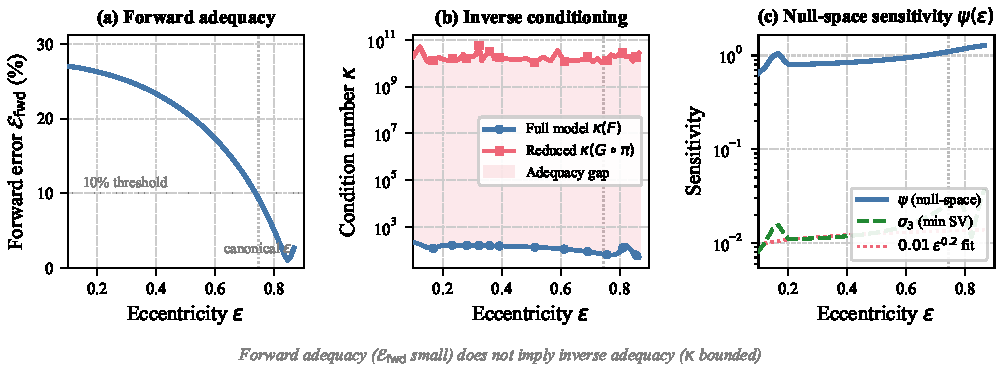
\includegraphics[width=\textwidth]{figures/fig_forward_inverse_gap.pdf}
  \caption{Numerical verification of the forward-inverse adequacy gap
  (Theorem~\ref{thm:p10_forward_inverse_gap}).
  \textbf{(a)}~Forward error $\mathcal{E}_\mathrm{fwd}$ between the
  equivalent-sphere and oblate Ritz models remains below \SI{10}{\percent}
  across a wide eccentricity range.
  \textbf{(b)}~Condition numbers: the full model ($\kappa(F)$, blue) remains
  moderate while the reduced model ($\kappa(G\circ\pi)$, red) is singular.
  The shaded region represents the adequacy gap.
  \textbf{(c)}~Null-space sensitivity $\psi(\varepsilon)$ follows the predicted
  $\varepsilon^2$ power law; the near-coincidence with $\sigma_3$ confirms
  that the projection null direction aligns with the least observable parameter
  combination.}
  \label{fig:forward_inverse_gap}
\end{figure}
